\section{国際SKAのサイエンス}\label{galaxy.s2}

%%%%%%%%%%%%%%%%%%%%%%%%%%%%%%%%%%%%%%%%%%%%%%%%%%%%%%%%%%%%%%%%%%%%%%%%%%
\subsection{水素原子吸収線系で探る銀河進化}
\label{subsec:international_21cm}
%%%%%%%%%%%%%%%%%%%%%%%%%%%%%%%%%%%%%%%%%%%%%%%%%%%%%%%%%%%%%%%%%%%%%%%%%%

国際的にも、クエーサー電波連続光を背景にして、視線方向にある
水素原子21 cm線吸収線を検出することにより、
銀河進化を研究する手法は注目されている。吸収線は輝線に比べて、
明るい背景光を
利用できるという利点があるために、再電離期までの遠方($z\sim 6$)に
わたってサンプルが取られることが期待される。
特に、活動銀河核(AGN)周りのガス-- \textit{associated absorber} (ここでは
「AGNに附随するガス」と呼ぶ)--の
運動をトレースする研究や、
遠方クエーサーの視線上にある中性水素雲-- \textit{intervening absorber}
(ここでは「吸収線系」と呼ぶ)--を
サンプルして銀河進化を調べる研究が挙げられる\citep{morganti14}。
以下に、AGNに附随するガスと吸収線系について、
どのような議論が国際サイエンスブックでなされているかを紹介する。

\paragraph{AGNに附随するガス}

H {\sc i}吸収はAGN周りのガスの物理状態をトレースするのにこれまでにも
使われてきた。例えば、Centaurus Aの電波源を背景にした21 cm吸収線の
検出は1970年に遡り\citep{1970ApJ...161L...9R}、核周辺を取り巻くガス
\citep{2008A&A...485L...5M,2012A&A...546A..22S}や
アウトフロー\citep{2013Sci...341.1082M}の運動が調べられている。
特に、後者の論文で観測された4C12.50のアウトフローは1000 km s$^{-1}$の
高速であり、質量放出率は$16-29$ $M_\odot$ yr$^{-1}$である。
エネルギーに換算すると降着エネルギーの$0.2-0.3\%$がアウトフローに
転換されている事になる。アウトフローばかりでなく、アウトフローのエネルギー源
に当るAGN中心のブラックホールへ降着しているガスの
インフローを捉える試みもなされているが\citep{1989AJ.....97..708V}、
降着円盤成分等との切り分けは容易ではない。

AGNに附随するH {\sc i}ガスに関する、H {\sc i}量、検出成功率、
ガスの運動、天体のタイプとの関係等は、Gerebら\citep{gereb14}に
よってまとめられている。彼らは$z=0.02$から0.23の電波AGNを
サンプルとし、それらの吸収線profileをスタッキングする事でより深い
検出限界に挑んだ。スタックしなくても検出できる
もの($N_\mathrm{HI}\sim 7\times 10^{20}$ cm$^{-2}$)が
あった一方、それ以外の検出できない
ものはスタックしても検出できなかった($N_\mathrm{HI}<2.26\times 10^{19}$ cm$^{-2}$)。
つまり、水素の柱密度に関して二極化の傾向がある事になる。また、コンパクトな
電波源の方が広がったものよりH {\sc i} 21 cm吸収が検出される傾向にあった。
これは、コンパクトな電波源の方がガスを多く持っている傾向がある事を示唆する。

AGNに附随する21 cm吸収は、$z\geq 0.1$では40天体、$z\geq 2$では僅か2天体で
ある\citep{1991PhRvL..67.3328U,1999ApJ...510L..87M}。高赤方偏移での検出が
少ないのは、高赤方偏移では可視域で明るいAGNに観測がバイアスしており、そのような
明るいAGNは周囲のガスを電離してしまうからであろうと考えられる\citep{2012ApJ...759..117C}。
SKAでは、暗い天体まで観測する事によって、バイアスは改善する事が期待される。
特に、SKAは広い視野を持つため、
サーベイ効率がいいので、ブラインドサーベイを実行できることからも、上記のバイアスは
低減されることが期待される。実際、SKA1では、およそ$z\sim 3$にまで届く感度が実現
される。SKAの前にも、ASKAPによって$z\sim 1$に近い所まで迫る事ができると
期待されている。

\paragraph{吸収線系}
遠方にある明るい電波源を使う事により、その手前にあるH {\sc i}雲の
21 cm吸収を検出する研究を行う事が出来る。そのような雲を21 cm吸収線系と
呼ぶ。これまでの21 cm吸収線系のサンプルは、ほぼ全てがLy$\alpha$の
吸収線系として知られているものをターゲットとして得られたものである。
それられの天体は、地上からLy$\alpha$が観測できる赤方偏移($z>2$)が対象となり、
ダスト減光の大きな雲はサンプルから漏れる傾向にある。SKAでは、
このバイアスを克服するために、連続光源自体を電波で探査し、これまでの
可視望遠鏡で得られていたサンプルとは独立のサンプルを取る事が
求められる。
SKA1では、$z\sim 3$まではSKA1-MIDもしくはSKA1-SURVEYで
$z$が3よりずっと大きなところはSKA1-LOWで観測できる。
SKA2では、21 cm吸収線系のブラインドサーベイが$z\sim 6$かそれを超える
赤方偏移まで可能であると見積られている\citep{2004NewAR..48.1259K}。

遠方銀河の中性水素に関して、過去10年の世界における研究の進展は
主として以下のようになる。
\begin{enumerate}
\item 電波CO輝線による分子ガスの観測は、近年のsubmm、mm波
干渉計の感度向上に伴って、遠方銀河まで出来るようになって来た。
近年の観測によれば、銀河の分子ガス量は、中性水素ガス量に比べて
概して$0<z<2$で急速に進化しているという結果が
ある\citep{2011MNRAS.418.1649L} (図\ref{fig:lagos})。しかし、
個々の銀河についてそれぞれ分子ガスと中性水素ガスの比を詳しく
観測する事はまだ出来ていない。これはALMAとSKAとの共同観測に
よって達成する事が期待される、SKA時代の新課題である。
準解析的モデル等によるモデル化も進みつつある\citep{2011MNRAS.418.1649L}
(図\ref{fig:lagos})。
\item DLAの21 cm線によるフォローアップ観測では、実は多くが
21 cmでは吸収されていない。この解釈は、大部分のDLAは、
スピン温度1000 K程度以上である事が分かっている\citep{2014MNRAS.438.2131K}。
(21 cm光学的厚さ$\tau$は、スピン温度の逆数に比例する事に注意。)
\end{enumerate}

SKA以前にも、以下のようなpathfinderによる観測が計画されている。
ASKAPによるFLASH(the First Large Absorption Survey in
H {\sc i})\footnote{http://www.caastro.org/research/evolving/flash}サーベイは南半天球全体の明るい($>$50 mJy)電波
連続光源(電波銀河とクエーサー) 150,000個の視線方向に
ある21 cm吸収線系を$0.5<z<1$の
範囲で探査する。この探査では、視野当り
2時間の積分時間で、1 Jyの背景光源に対して$\tau\sim 0.01$の
光学的厚さが5 $\sigma$で検出でき、
最も暗い(50 mJy)の光源に対しては$\tau\sim 0.3$である。
ApertifとMEERKATによるサーベイでは、より小さい天域に絞って
より深い観測を行う事が計画されている。

\begin{figure}[tbp]
\begin{center}
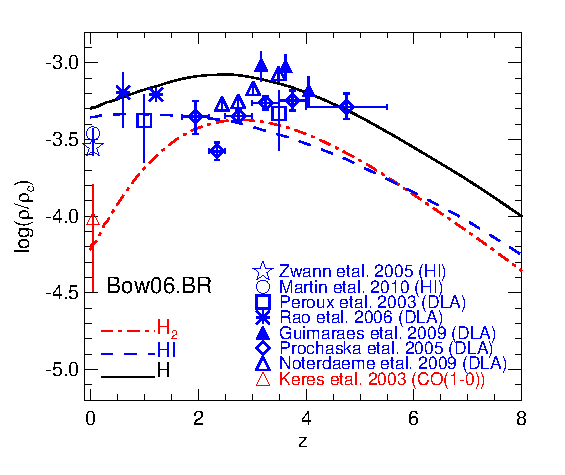
\includegraphics[width=0.7\linewidth]{galaxy/lagos_HI_H2a.eps}
\end{center}
\vspace{-1cm}
\caption{論文\citep{2011MNRAS.418.1649L}より転載。
準解析的モデルから予想される全ての電離していない
水素(実線)、水素原子(破線)、水素分子(鎖線)の
宇宙全体での密度を宇宙の臨界密度で規格化したもの
の赤方偏移進化。観測データは青($z=0$の三角以外)は
水素原子、赤($z=0$の三角)は水素分子の観測をプロット
している。}
\label{fig:lagos}
\end{figure}

SKA1で提案されている10,000平方度のサーベイを行うと、
30 mJy程度の明るさの背景光源に関しては
5 $\sigma$の検出限界で$\tau\sim 0.015$程度のものまで観測できる
(10 mJyの背景光源では$\tau\sim 0.05$、2--3 mJyのものでは
$\tau\sim 0.1$)。全部で数千個規模の21 cm吸収線系のサンプルが
$z=3$程度にまでわたって得られると期待される。

\subsection{電波再結合線で探る冷たい中性水素雲}

水素21 cm線だけが中性(電離度が低い)雲を見る電波のトレーサーではない。
電波($<350$ MHz)での炭素や水素の電波再結合線を観測する事で、
冷たい中性雲をトレースする可能性も検討されている\citep{oonk14}。
冷たい中性雲は、宇宙線によって少し電離しており、その電波再結合線を
捉えるのである。それにより、冷たい中性ガス
(CNM)の温度、電離度、
炭素の存在比等が分かる。\ref{subsec:international_21cm}節で述べた
中性水素21 cm線だけでは区別できないcold、warmの二相を、電波再結合線
がcoldのみで検出できる事を使うと区別できる。

Low Frequency Array (LOFAR)で、系外電波源Cygnus A (Cyg A)を
背景光として、電波再結合線を吸収線で検出した最初の例が
図\ref{fig:oonk}に示されている。ただし、再結合線自体は
銀河系の中性ガスに由来するものが検出されている。
電子温度110 Kと電子数密度
0.06 cm$^{-3}$が観測から導かれている。Cygnus Aに附随する
H {\sc i}ガスの光学的厚さは、4 km s$^{-1}$の速度分解能で
3 $\sigma$の上限$\tau_\mathrm{HI}^{3\sigma\text{upper}}=1.5\times 10^{-4}$が得られている。SKAでは系外の
中性ガスの吸収を遠方の電波源を用いて観測できることが
期待される。

銀河系の電波再結合線の観測も当然
SKAで推進できる\citep{oonk14}が、ここでは系外銀河の
観測に焦点を絞る。最近、LOFARにより、系外銀河M82の炭素電波再結合線が
検出された。これは、電波再結合線が冷たい中性水素ガスのトレーサーとして
観測的に使える可能性を拓くものである。

電波銀河を背景光源として用いることにより、SKAでは電波再結合線を吸収線で
$z=0$から5にわたって検出できると期待される。LOFARでも比較的近傍の数百個程度
の電波銀河を背景光源として使う事ができるが、SKA1-LOWでは$10^5$個程度にまで
増えると期待される\citep{oonk14}。同一の吸収天体による複数の電波再結合線を
同定する事で、その天体の赤方偏移も割出す事が出来る。
また、近傍銀河なら、それ自体の電波放射を背景光源とした電波再結合線も
検出できる。SKA1-LOWでは500個程度の近傍星形成銀河が電波再結合線で
観測できると期待されている(SKA2では3000個程度)。

\begin{figure}[tbp]
\begin{center}
\includegraphics[width=0.6\linewidth,angle=90]{galaxy/oonk_rrl.eps}
\end{center}
\caption{論文\citep{2014MNRAS.437.3506O}より転載。
銀河系の電波再結合線を系外電波源を背景にして検出した最初の
例。LOFARによる。33--57 MHzにある48個の炭素$\alpha$線を
スタッキングし、得られたスペクトル。
黒い実線はデータ、赤い破線はガウシアンでフィットした
結果。}
\label{fig:oonk}
\end{figure}



%%%%%%%%%%%%%%%%%%%%%%%%%%%%%%%%%%%%%%%%%%%%%%%%%%%%%%%%%%%%%%%%%%%%%%%%%%
\subsection{電波連続波で探る銀河進化}
\label{subsec:international_cont}
%%%%%%%%%%%%%%%%%%%%%%%%%%%%%%%%%%%%%%%%%%%%%%%%%%%%%%%%%%%%%%%%%%%%%%%%%%

\ref{galaxy.s1}節で述べた様に、銀河の電波連続波の光度は星形成率の
良い指標である。特に、紫外・可視域の星形成率指標(紫外連続光光度、
バルマー系列輝線光度等)に比べると
ダスト減光の影響がないという利点がある。また、ダストの赤外放射光度も
星形成率の良い指標であることが知られて
いる\citep[e.g., ][]{1998ARA&A..36..189K,2000PASJ...52..539I}が、ダストが極端に
少ない環境では星形成活動指標として使えないことが予想
される\citep{2001A&A...366...83H}。一方で、
電波連続波はダストのない環境でも星形成率指標として利用できる点で
ダストの影響を受けない星形成活動指標と言える。

\color{red}
また、電波連続線によるサーベイでは活動銀河核(AGN)の一種である電波銀河が明るい側で卓越した成分として現れるという特徴がある。電波銀河は、銀河中心の超巨大ブラックホール(SMBH)からの高エネルギージェット及びMpcスケールの巨大なローブから放射される強力なシンクロトロン放射が特徴的である。この放射強度は典型的に星形成銀河の100倍程度であるため、通常の星形成活動起源の電波放射とは分離される。電波銀河は降着の最終期また、inter cluster medium (ICM)への物質輸送も行われる。そのため、AGNはSMBHへの物質降着に起因する減少であるため、電波銀河の電波放射の赤方偏移進化を探ることで銀河-ブラックホール共進化が銀河進化に果たしてきた役割の示唆を得ることができる。
\color{black}

ここでは国際サイエンスブックの
\citet{murphy15}に基づき、SKAへ向けて国際的にどのような
観測が検討されているかを紹介する。彼らは特に、ultra-deep SKA1-MID/Band 5
reference survey \citep{prandoni15}に着目している。Band 5の周波数域は
4.6--13.8 GHzである。

従来、電波域の銀河サーベイの周波数は低周波、特に1.4 GHzでの
サーベイが、視野(primary beam)が大きい点とシンクロトロン放射強度が
周波数に対して負冪の依存性を持っている(つまり、低周波になると
銀河が明るくなる)点で有利であったので、主流であった。
例えば、\citet{2008MNRAS.386.1695S}
では、Multi-Element Radio-LInked Network (MERLIN)とJansky Very Large Array (JVLA)の
1.4 GHzの観測とJVLAの4.8 GHzの観測を用いて、$z<3$での宇宙の星形成史を
導き、可視域等で得られたものと整合的な値が
得られた(\citealt{2010ApJS..188..178M}も参照)。また、
\citet{2009ApJ...690..610S}
では、JVLA 1.4 GHzの観測により、$z=1.3$までの電波連続波光度関数の進化を
観測的に明らかにした。ただし、感度の関係から光度関数の高光度側に
基づいて議論が構築されている。

\color{red}
さらに近年では、COSMOS領域においてJVLAを用いて3GHzにおけるさらに深い($F_{\rm lim}=11.7 {\rm \ \mu Jy}$)サーベイ(VLA-COSMOS 3GHz Large Project)が行われた\cite{2017A&A....602...A1}。
このサーベイに基づいて、星形成銀河とAGNについて$z \leq 6$における電波光度関数の進化モデルが構築された\citep[e.g., ][]{2017A&A....602...A6, 2017A&A....602...A5, 2018A&A....614...47N}。
特に、星形成銀河については紫外線や赤外線といった他の星形成指標から得られた星形成史との比較がなされており、銀河形成期から現在に至るまでこれらの波長帯と整合的な結果が得られる事が確認されている。ただし、感度による制限から星形成銀河電波光度関数の暗い側についての傾きは依然として定められていない。
銀河中の星形成は宇宙再電離の主要因であると考えられている\citep[e.g., ][]{2016MNRAS....463...1968Y}ため、高い感度の観測によって光度関数の暗い側のパラメータについてより厳しい制限が付けられることが今後求められる。
また、電波銀河と異なり、母銀河からの熱的放射が電波放射の大半を占めるAGNの種族であるRadio-Quiet AGN (RQ AGN)についても、電波帯における暗さから進化を議論している研究は少ない\citep[e.g., ][]{2011ApJ...740...20P, 2015MNRAS...452...1263P}ため、SKAによる更新が期待される。
SKA1では0.12GHz (SKA1-low)においてVLA-COSMOSと同程度の感度である$20\ {\rm \mu Jy}$におけるAll-skyサーベイ、1GHz (MID Band 1 and/or 2)において$F_{\rm lim}=50 {\rm \ nJy}$の感度による$1 {\rm deg}^2$にわたるUltra-deepサーベイなどが計画されている\cite{prandoni15}ため、銀河形成・進化についてより詳細な描像が得られると考えられる。
また、電波連続波による銀河計数についての近年の理論的な研究には\cite{2017ApJ....842...95}, \cite{2017MNRAS...469...4083S}が挙げられる。特に、\cite{2017ApJ....842...95}では銀河の星形成活動がSMBHによるフィードバックによって抑制されるまでの各物理過程のタイムスケールを評価することで、銀河種族ごとの赤方偏移分布について解析的なモデル構築を行っている。
ここでも、SKAによる低振動数電波観測によって検出される銀河計数の評価を行っている。
\color{black}


\citet{murphy15}がSKAで着目しているサーベイは比較的高周波に着目している点に特徴がある。
SKAではその高感度から、$\gtrsim 10$ GHzでも、従来の
電波望遠鏡に比べると格段に高いサーベイ効率で
銀河サーベイを行う事ができる。Band 5では、SKA1-MID、SKA2では
それぞれ1平方度当り約30、85個の銀河が検出できると見積られる。
10 GHzもしくはそれ以上の高周波は、
以下の2点で科学的利点がある: (i)
より高い角分解能で観測できる。特に、200 kmのベースラインが取れれば、
10 GHz以上の周波数での観測は、各分解能0.03秒角以下を達成でき、
これは則ち、$z\gtrsim 1$にある銀河でも250 pcスケールが分解できる事を
意味する。また、この分解能は、可視・近赤外域で計画されている\textit{JWST}等
の分解能とも良くマッチしている。(ii) 高周波で卓越するfree--free放射は、
低周波で卓越するシンクロトロン放射に比べて、大質量星からの
電離光子放射光度を直接的に反映する点で現在の星形成活動を
良くトレースしている。特に高赤方偏移では、
シンクロトロン放射を担う高エネルギー電子は、
宇宙背景放射を逆コンプトン散乱してエネルギーを失う傾向にあるので、
シンクロトロン放射は星形成活動のトレーサーとして使えない可能性がある。
これらの二点に基づき、彼らはSKAでの10 GHz以上の周波数域を
強く要求している。特に、
30 GHzまで周波数域を拡張することにより、ALMAと
周波長が連続的に取れる面でも、科学的メリットが大きいと主張する。

特に、free--free放射の重要性は、若いスターバースト\color{red}銀河\color{black}で顕著になる。
近傍の若いスターバーストの電波スペクトルは、
free--free\color{red}放射\color{black}が卓越していると解釈できるフラットな周波数依存性を持つという
結果が得られている\citep{1993ApJ...410..626D,2003ApJ...593..733R,2005A&A...436..837H}。
電波スペクトルの年齢依存性は、高赤方偏移ではとりわけまだ定まった結論を得るに
至っていない: 遠方のスターバースト\color{red}銀河\color{black}のいくつかはフラットな電波
連続波スペクトルを
持つ\citep{2005A&A...436..837H,2006A&A...460...67H,2011MNRAS.415.3473V}のに
対し、反対の傾向を持つ遠方銀河も
ある\citep{2011MNRAS.410.1155B,2014MNRAS.442..577T}。
広帯域を持つSKAでは、電波スペクトルの形(特にspectral index)を
様々な赤方偏移で決めるのに適しているので、電波連続波スペクトルの
年齢(もしくは赤方偏移)に依る進化を明らかにするのに適している。
特に、10 GHz以上の周波数域が観測できる事が理想的である。

シンクロトロン放射自体も、超新星等に伴う星間空間での高エネルギー過程を
トレースする重要性があるので、理解を欠かす事はできない。また、
星間磁場の強さや進化に対する制限も得られる可能性があり、free--free\color{red}放射\color{black}成分に
勝るとも劣らず重要である事も強調しておかねばならない。
シンクロトロン\color{red}放射\color{black}とfree--free\color{red}放射\color{black}の両方を観測できるSKAの広帯域は、
この点でも魅力的である。

最後に、連続波以外にも、
30 GHzまで周波数域を拡張する利点は幾つかある。
表\ref{tab:summary_line}ではバンドの上限周波数は
10 GHzを仮定したが、30 GHzまで拡張されれば、AGNのH$_2$Oメーザーの
観測が近傍銀河でも
可能になる。また、CO ($J=$ 1--0)も$z>2.8$で
観測可能となる。つまり、重要な輝線の観測範囲が低赤方偏移へ
降りてくる。ALMAとシームレスに繋がる点も再度強調しておく。

